Roadmap:
\begin{itemize}
    \item räumliche und zeitliche Kohärenz
    \item MM Interferoeter, g1
    \item van Zittert Cernike -> Blendengeometrie; Wiener Khinchin -> Spektrum
    \item Intensitäteninterferometrie g2, Siegert Relation
    \item thermisches und chaotisches Licht, bunching anhand von g2
    \item g2(0) <2 erklären
\end{itemize}

\subsection{Kohärenz}
\label{ssec:Kohärenz}
Um ein stabiles Interferenzmuster beobachten zu können, ist es wichtig dass die beiden einfallenden Lichtfelder eine feste Phasenbeziehung zueinander haben. 
Ist dies nicht der Fall, überlagern sich verschiedene Interferenzmaxima und -minima und ergeben ein räumlich und zeiltich unstetiges Muster. 
Um diese Eigenschaft des Lichts besser zu beschreiben, gibt es den Begriff der Kohärenz.
Man unterscheidet zwischen räumlicher und zeitlicher Kohärenz, wobei räumliche die Phasenbeziehung an verschiedenen Orten der selben Wellenfront und die zeitliche Kohärenz die Phasenbeziehung an ein und demselben Ort, aber zu verschiedenen Zeiten quantifiziert.
Eine veranschaulichende Skizze ist in \autoref{fig:skizze kohärenz} dargestellt.
\begin{figure}[htbp]
    \centering
    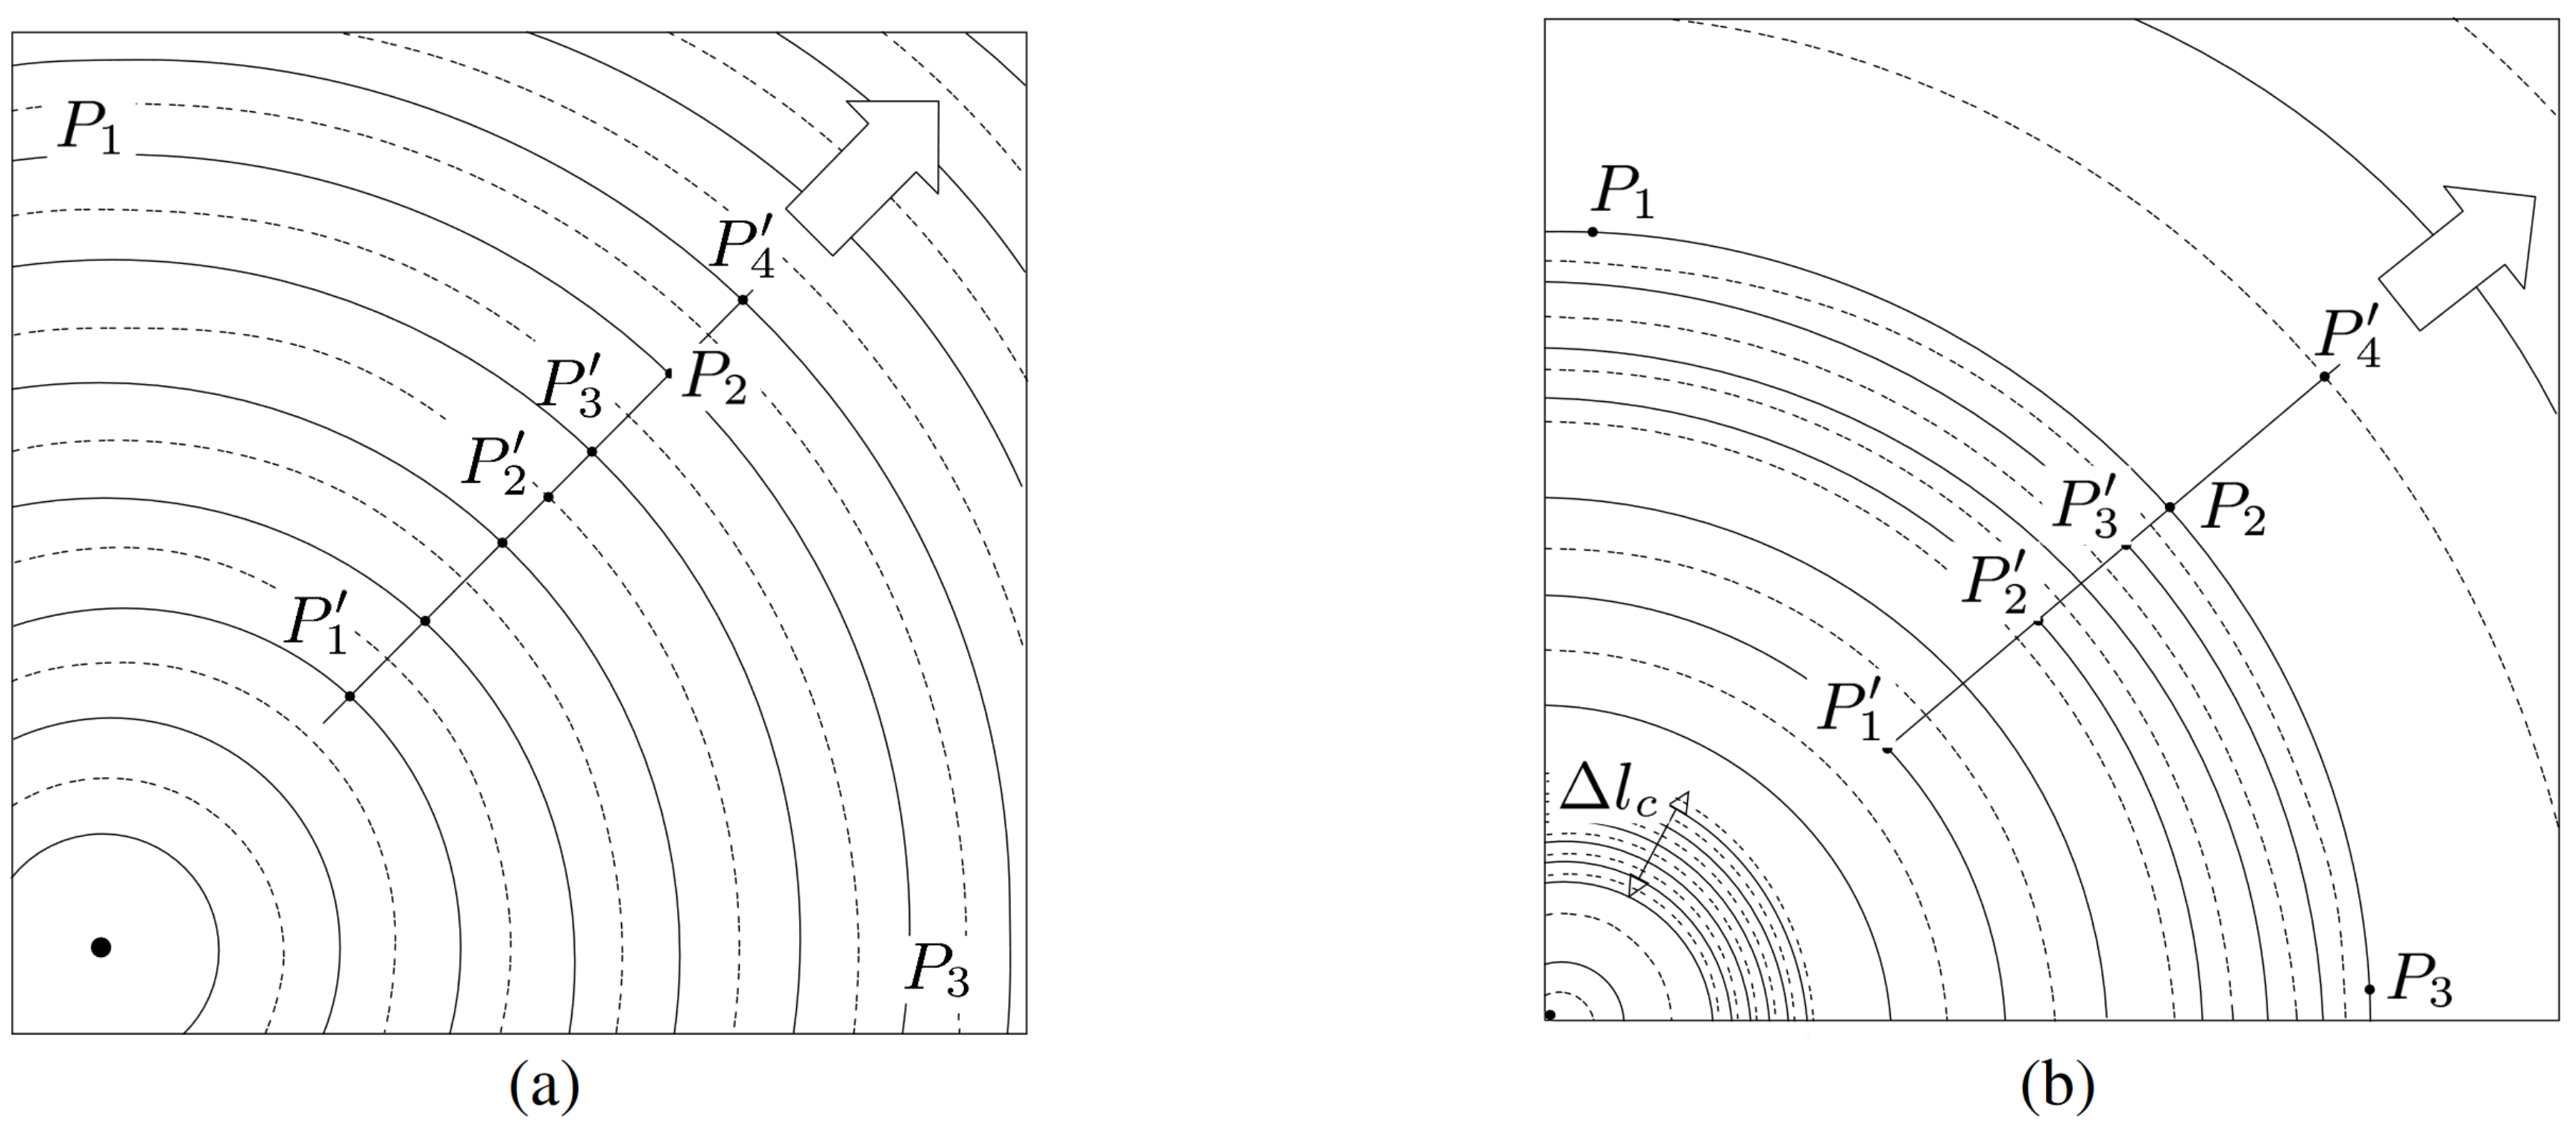
\includegraphics[width=0.8\textwidth]{images/Theorie/Hecht_9.6.png}
    \caption{Dargestellt ist eine Skizze von Wellenfronten zur Veranschaulichung von Kohärenz. In (a) ist die Welle vollständig räumlich und zeitlich kohärent. In (b) ist die Welle nur noch teilweise zeitlich kohärent, aber weitherhin räumlich kohärent. Die Kohärenzläge $\Delta l_c$ ist eingeziechnet. Abbildung entnommen aus \cite{hecht_optik_2018}.}
    \label{fig:skizze kohärenz}
\end{figure}
\autoref{fig:skizze kohärenz} a zeigt eine vollständig kohärente Welle. Die Phasenbeziehung zwischen Punkten in Ausbreitungsrichtung ist vollkommen deterministisch, die Welle ist monochromatisch und damit zeitlich, oder longitudinal kohärent. 
Auch in transversaler Richtung (vergleiche Punkte $P_1$-$P_3$) entlang einer Wellenfront ist die Phasenbeziehung für jeden Zeitpukt identisch. 
Die Welle ist räumlich oder transversal kohärent. 
Räumliche Kohärenz liegt auch in \autoref{fig:skizze kohärenz} (b) vor. 
Allerdings ist erkennbar, dass die Welle in longitudinaler Richutung nicht für alle Distanzen eine feste Phasenbeziehung hat. 
So ist die Frequenz in $P_1'$ z.B. niedriger, als die in $P_3'$. 
Allerdings existieren trotzdem Bereiche, in welchen die Phase sich deterministisch verändert. 
Die kürzeste Länge für die dies gilt, ist die Kohärenzlänge $\Delta l_c$, die über die Ausbreitungsgeschwindigkeit $c$ mit der sog. Kohärenzzeit $\Delta l_c = c\tau_C$ zusammenhängt. 
Die Kohärenzzeit ist damit jene Zeit, für welche die Phase einer Welle vorhersehbar ist. 
Damit haben vollständig zeitlich kohärente Quellen eine unendlich lange, teilweise kohärente Quellen eine endliche Kohärenzzeit und für inkohärente Quellen gilt $\tau_c =0$. 

Aus der obigen Abbildung wird direkt erkenntlich, dass die Kohärenzzeit ein Maß für die spektrale Breite des Lichts $\Delta \omega$ darstellt. 
Es gilt \cite{fox_quantum_2006}:
\begin{equation}
    \tau_c  \approx \frac{1}{\Delta \omega}
\end{equation}
Da Kohärenz eine Korrelation in den Feldamplituden beschreibt, lässt sich diese Eigenschaft des Lichtes mathematisch auch mit der sog. Korrelationsfuntion erster Ordnung beschreiben. 
Diese lautet \cite{foellmi_intensity_2009}:
\begin{equation}
    g^{(1)}(\mathbf{r_1}, t_1, \mathbf{r_2}, t_2) = \frac{\left<E^*(\mathbf{r_1}, t_1)E(\mathbf{r_2}, t_2)\right>}{\left[\left<E^*(\mathbf{r_1}, t_1)^2\right> \left<E(\mathbf{r_2}, t_2)^2\right>\right]^{1/2}}
    \label{eq:g1(r,t)}
\end{equation}
Hierbei bezeichnet $E_i(\mathbf{r_i},t_i)$ die komplexe Feldamplitude am Ort $i$ und $\left<\dots\right>$ den Zeitmittelwert über eine lange Zeit. 

% Todo:
% g1 umschrieben (quelle finden) 